%!TEX root = ../my_thesis.tex

\newcommand{\curChapter}{main/chapter1}

\chapter{Context and Objectives}
\label{chap:ctx}

This chapter introduces the context of digital communication systems. Its
purpose is to define notions that will be reused in the manuscript and to give
a general view and defines the main objectives of this thesis. The first section
presents the principle of the digital communication systems with its different
parts: transmitter, channel and receiver. The most common metrics used in
digital communications are also introduced. The second section details the
channel model and the digital modulation used all along the manuscript. A
characterization of the signal-to-noise ratio is given as well as the notion of
probability at the output of the channel and the demodulator. The third section
introduces the channel codes considered in this manuscript: namely the LDPC, the
polar and the turbo codes. The corresponding encoding and decoding processing
are detailed for each channel code family. In the fourth section, three
applicative contexts are detailed for the considered channel codes. The
functional simulation enables the design and the validation of a coding scheme.
The software-defined radio is a radio communication system where components are
implemented by means of software. Then, the sparse code multiple access
mechanism is presented as it is a promising solution for massive connectivity in
future mobile networks. The fifth section gives the main problematics of the
thesis.

\vspace*{\fill}
\minitoccustom
\vspace*{\fill}

\section{Digital Communication Systems}
\label{sec:ctx_digital_communication_systems}

\begin{figure}[htp]
  \centering
  \includegraphics[scale=1.0]{\curChapter/fig/intro/com_chain/com_chain}
  \caption{Digital communication chain.}
  \label{fig:ctx_com_chain}
\end{figure}

It is now commonplace to state that Humanity has entered the era of
communication. By 2025, there should be more than 5 billion smart-phones in
circulation worldwide. Moreover, all kinds of objects will increasingly use
communication technology, to exchange information in the \emph{Internet of
Things} (IoT), for instance. Despite their heterogeneity, all communication
systems are based on a common abstract model proposed by Claude Shannon. In his
seminal paper~\cite{Shannon1948}, he proposed to model a communication system
with five major components: an information source, a transmitter, a channel, a
receiver and a destination. This model was later refined as shown in
Figure~\ref{fig:ctx_com_chain}. The source produces a digital message $\bm{u}$
to be transmitted (sequence of bits). The channel encoder transforms it in a
codeword $\bm{c}$ to make it more robust to errors. In order to make possible
the information transmission through the channel, it is necessary to shape the
data stream. For instance, in the case of wireless communication, this stream
must be represented by a high-frequency signal in order to be transmitted by a
reasonably sized antenna. This is the role of the digital modulator which
produces a vector of symbols $\bm{x}$. The channel alters the signal with some
noise and distortions ($\bm{y}$). On the receiver side, the components perform
the inverse operations to retrieve the decoded message $\bm{\hat{u}}$. If no
errors occurred during the transmission or if there is errors but they have been
corrected, $\bm{\hat{u}} = \bm{u}$.

In the next sections and chapters, we will focus on channel coding because it
comes with algorithms that have the highest computational complexity in the
digital communication systems. In channel coding, also known as \emph{forward
error correction} (FEC), $K$~information bits  are encoded in the transmitter.
It results in a codeword $\bm{c}$ of $N$ bits. $P = N - K$ is the number of
redundancy bits added as additional information and $R = K/N$ is the code rate.
The higher the code rate $R$ is, the lower the number of bits $P$ is. The
performance of this scheme is measured by estimating the residual error rate at
the sink. It is possible to observe two different rates: 1) the Bit Error Rate
(BER); 2) the Frame Error Rate (FER). The BER is calculated considering the $K$
information bits independently, for instance a $10^{-3}$ BER means that there is
an average of one binary error per thousand information bits transmitted. The
FER is computed considering the entire frame, if there is at least one wrong bit
in the current frame, it will be counted as one erroneous frame. A $10^{-2}$ FER
means that there is an average of one frame error per hundred frame transmitted.
These rates depend on many factors: the noise of the channel, the modulation
type, the code type, the code rate $R$, etc. The lower the bit and frame error
rates are, the higher the correction power of the system is.

\section{Channel Model}
\label{sec:ctx_awgn}

In this thesis, only causal transmission channels without memory effect and
stationary are considered. In other words, the output of the channel at time~$t$
only depends on its input at time $t$. In order to describe the disturbance
applied to the message $\bm{x}$ passing through the transmission channel,
different models can be used. However, in the literature, the selected model is
often the Additive White Gaussian Noise (AWGN) channel. In particular, this
channel well models the thermal noise which is one of the sources of noise
that is always present on the receiver side. This section presents the AWGN
channel concepts and introduces the Binary Phase-Shift Keying
modulation/demodulation that is employed all along the manuscript.

In the AWGN channel, the law binding the $y_i$ output to its $x_i$ input is of
the form $y_i = x_i + n_i$ with $N_{chn}$ an independent and identically
distributed variable according to a normal (or Gaussian) law centered in zero
and of variance $\sigma^2 = N_0 / 2$. So, we have $N_{chn} \simeq \mathcal{N}(0,
\sigma^2)$ and:
\begin{equation}
P(y_i|x_i) = \frac{1}{\sqrt{2\pi}\sigma}\exp{\Big(-\frac{(y_i-x_i)^2}{2\sigma^2}\Big)}.
\end{equation}

To estimate the correction power of a channel code it is very common to vary the
Signal-to-Noise Ratio (SNR). On the AWGN channel the SNR is generally given by
$E_b/N_0$ (in dB). $E_b$ corresponds to the average energy per information bit.
It can also be given by $E_s/N_0$ (in dB) where $E_s$ corresponds to the average
energy per transmitted symbol. A symbol is a binary or a non-binary quantity, so
it can be represented by one or more bits. $E_s/N_0$ can be deduced from
$E_b/N_0$ as follows:
\begin{equation}
\frac{E_s}{N_0} = \frac{E_b}{N_0} + 10.\log{(R.b_S)},
\end{equation}
where $R$ is the code rate and $b_S$ is the number of bits per transmitted
symbol $x_n$. $b_S$ depends on the modulation order. If a binary modulation is
used, then $b_S = 1$. The channel variance is:
\begin{equation}
\sigma = \sqrt{\frac{1}{2 \times 10^{\frac{E_s}{N_0} / 10}}}.
\end{equation}

An important characteristic of a channel is its capacity~\cite{Shannon1948}. The
capacity represents the maximal quantity of information that the canal can
transport. In other words, it is impossible to find a coding scheme that
transports more information than the channel capacity. From this capacity it is
possible to deduce Shannon's limit. This limit is the asymptotic SNR in
$E_b/N_0$ (dB) which cannot be improved with any channel code. When $R$ tends
towards zero it can be shown that Shannon's limit is $-1.59$ dB. This means
that, for an AWGN channel, no system can reliably transmit information at an SNR
of less than $-1.59$ dB.

In the next chapters of the manuscript, the AWGN channel will mainly be
associated with a Binary Phase-Shift Keying (BPSK) modulation ($b_S = 1$). With
this modulation, each binary value $c_i \in \{0,1\}$ is associated to a real
value $x_i \in \{1,-1\}.$ The $\bm{l}$ outputs estimated by the digital
demodulator can be given in the form of a Log Likelihood Ratio (LLR). Their sign
determines for each channel output data $y_i \in \bm{y}$ the most likely binary
input $c_i \in \bm{c}$. The absolute value corresponds to the degree of
reliability of the information. The mathematical expression of $l_i$ is:
\begin{equation*}
l_i = \log{\Big(\frac{P(y_i|c_i = 0)}{P(y_i|c_i = 1)}\Big)}.
\end{equation*}

\section{Channel Codes}

After Shannon's work, researchers have designed new coding/decoding schemes to
approach Shannon's theoretical limit increasingly closer. Indeed, recent
progresses managed to design practical codes performing very close to that
limit. These codes are already integrated in current communication systems. They
are usually classified in two main families: block codes and convolutional
codes. The block codes generate the redundancy by packets of data while the
convolutional codes compute the redundancy bit by bit on the data stream. The
purpose of this section is to introduce the most used channel code families.

The convolutional codes have been introduced by Peter Elias in
1955~\cite{Elias1955}. The objective was to propose an alternative to the block
codes in term of codeword length flexibility: theoretically the length of a
convolutional code is infinite. The coding scheme is made in a way that the
output depends on the current input and on the inputs before. This type of code
has been used by the NASA for satellite communications for instance.

The Raj \textbf{B}ose, D. K. Ray-\textbf{C}haudhuri and Alexis
\textbf{H}ocquenghem (BCH) codes are block codes discovered in the late
1950s~\cite{Hocquenghem1959,Bose1960}. They are algebraic codes built from a
polynomial. This results in low complexity decoding algorithms. These codes are
used in the CDs, DVDs and SSDs. In modern coding schemes, they are often
concatenated to other codes in order to improve their correction powers
especially when there are erroneous frames with a small number of erroneous
bits. This is the case in the DVB-S2 standard for instance.

The Irving S. \textbf{R}eed and Gustave \textbf{S}olomon (RS) codes have been
proposed in 1960~\cite{Reed1960}. Like the BCH codes they are algebraic codes.
But unlike the BCH codes, the RS codes are based on symbols instead of bits
(non-binary codes). The RS codes are used in many standards (CD, DVD, Blu-ray,
ADSL, DVB-T, etc.).

The Low-Density Parity-Check (LDPC) codes are linear block codes. They have been
discovered by Robert G. Gallager in 1962~\cite{Gallager1962}. Unfortunately, at
the time of their discovery, the computational power available in the
transceivers was not sufficient to decode them. Later, in 1995, the LDPC codes
have been re-discovered by David MacKay~\cite{MacKay1995}. Nowadays, they are
used in many digital communication standards such as Wi-Fi, WiMAX, WRAN, 10Gbps
Ethernet, DVB-S2, CCSDS, 5G data transport, etc.

The turbo codes have been discovered by Claude Berrou in 1993~\cite{Berrou1993}
and have been used in many digital wireless communication standards since (3G,
4G, DVB-RCS2, CCSDS, etc.). The particularity of the turbo codes is to be
composed by two convolutional sub-codes. In other terms, the turbo codes are a
parallel concatenation of two convolutional codes.

The Turbo Product Codes (TPC) are block codes, they have been invented by Peter
Elias in 1954~\cite{Elias1954} while the first efficient decoding algorithm has
been discovered later in 1994 by Ramesh Pyndiah~\cite{Pyndiah1994}. A TPC is a
form of serial concatenation of two block codes, it results in a matrix where
one code can be read from the columns and the other one from the rows. The TPC
are notably used in the WiMAX standard and also in some optical communication
systems.

The polar codes are linear block codes like the LDPC. They have been invented
by \Arikan in 2009~\cite{Arikan2009}. For the first time, they are present in
the 5G standard (control channels). The particularity of these codes is that
they are the only ones for which it has been mathematically demonstrated that
they reach Shannon's limit (considering an infinite codeword length).

Many other codes exist like Hamming codes, Plotkin codes, Gilbert codes, Golay
codes, Reed-Muller codes~\cite{Muller1954,Reed1954}, the raptor
codes~\cite{Shokrollahi2004}, etc. The purpose of this section is not to be
exhaustive but to give a representative overview of the FEC domain. This thesis
will focus on a subset of these codes, namely the LDPC codes, the polar codes
and the turbo codes. These codes have been selected because they are known to
be channel capacity-approaching and well-spread in the current digital
communication standards. Moreover, these code families lead to high
computational complexity decoders that are challenging to implement.

\subsection{Prerequisites}

\begin{table}[htp]
  \centering
  \caption{Elementary operations in $GF_2$ (logical \emph{exclusive or} and
    logical \emph{and}).}
  \label{tab:ctx_gf2_operations}
   \begin{tabular}{c c c c}
   $a$ & $b$ & $a \oplus b$ & $ab$ \\
    \hline
    \hline
    0 & 0 & 0 & 0 \\
    0 & 1 & 1 & 0 \\
    1 & 0 & 1 & 0 \\
    1 & 1 & 0 & 1 \\
  \end{tabular}
\end{table}

In all the presented coding schemes, only binary codes are considered. In this
case, a bit can be represented in a Galois field of two elements $\{0, 1\}$
denoted as $GF_2$. A block code is an application $g$ of $GF_2^K$ in $GF_2^N$
with $K < N$. There are $2^K$ codewords $\bm{c}$. The two operations used to
generate a codeword are the addition and the multiplication. In $GF_2$, the
addition is equivalent to a logical \emph{exclusive or} ($\oplus$) and
the multiplication is equivalent to a logical \emph{and} (see
Table~\ref{tab:ctx_gf2_operations}).

In this chapter, all the decoding algorithms are working on \emph{soft}
information. This means that the decoding input is a vector of $N$ likelihoods
in the form of LLRs. Each LLR is a real value. Depending on the implementation
it can be a floating-point or a fixed-point number. It results in more complex
operations than for the encoding process. On the decoding side and in the
logarithmic domain, the $\oplus$ operator can become the $\boxplus$ operator, it
is defined as follow:
\begin{equation}
  l_a \boxplus l_b = 2\tanh^{-1}{\big(\tanh{(\frac{l_a}{2}).\tanh{(\frac{l_b}{2})}}\big)}.
\end{equation}
This is the main reason why, in channel coding, the decoders are systematically
more compute intensive than the encoders. In the logarithmic domain, the
multiplication becomes a simple addition.

\subsection{Low-density Parity-check Codes}
\label{sec:ctx_ldpc}

\subsubsection{Coding Scheme}

A parity-check constraint is an equation that links a set of bits: when all the
bits of a parity-check constraint are added together the result has to be
zero. For instance, if we consider a message $\bm{u} = [u_0, u_1, u_2, u_3]$
($K = 4$), then it is possible to encode the information message $\bm{u}$ in a
codeword $\bm{c}$ of size $N = K + 1 = 5$: $\bm{c} = [u_0,u_1,u_2,u_3,p_0]$.
The parity-check constraint $\mathcal{C}_0$ is then: $u_0 \oplus u_1 \oplus u_2
\oplus u_3 \oplus p_0 = 0~(\mathcal{C}_0)$ with $p_0$ the parity bit ($P = N -
K = 1)$. To encode the message $\bm{u}$ and produce the codeword $\bm{c}$, a
generator matrix $\bm{\mathcal{G}}$ (or a linear application) has to be defined
like this: $\bm{c} = \bm{u} \times \bm{\mathcal{G}}$ with
\begin{equation*}
\bm{\mathcal{G}} =
\begin{bmatrix}
1 & 0 & 0 & 0 & 1\\
0 & 1 & 0 & 0 & 1\\
0 & 0 & 1 & 0 & 1\\
0 & 0 & 0 & 1 & 1\\
\end{bmatrix}
.
\end{equation*}
$\bm{u} \times \bm{\mathcal{G}} = [u_0,u_1,u_2,u_3,u_0 \oplus u_1 \oplus u_2
\oplus u_3] = \bm{c}$, so $p_0 = u_0 \oplus u_1 \oplus u_2 \oplus u_3$ as
defined by the parity-check constraint $\mathcal{C}_0$. The proposed
generator matrix $\bm{\mathcal{G}}$ is composed by the identity matrix on the
four first columns and by the parity-check constraint in the last column.
The consequence of the presence of the identity matrix is that the generated
codeword contains the initial information bits $u_0$, $u_1$, $u_2$, and $u_3$.
In this case, the encoding process is \emph{systematic}.

\begin{figure}[htp]
  \centering
  \includegraphics{\curChapter/fig/ldpc/parity_check/parity_check}
  \caption{Representation of the $\mathcal{C}_0$ parity-check constraint on a
    Tanner graph.}
  \label{fig:ctx_ldpc_parity_check}
\end{figure}

One can note that a parity-check constraint can also be represented with a
Tanner graph as shown in Figure~\ref{fig:ctx_ldpc_parity_check}. It is also
possible to define a matrix of parity-check constraints namely
$\bm{\mathcal{H}}$. In this case, there is only one constraint
($\mathcal{C}_0$), so $\bm{\mathcal{H}}$ is a one-dimension matrix (or a vector)
of size $N$:
$
\bm{\mathcal{H}} =
\begin{bmatrix}
1 & 1 & 1 & 1 & 1
\end{bmatrix}.
$
An important property of the $\bm{\mathcal{H}}$ matrix is that it must satisfy:
$\bm{\mathcal{G}} \times \bm{\mathcal{H}}^T = \bm{0}.$

\begin{figure}[htp]
  \centering
  \includegraphics{\curChapter/fig/ldpc/parity_checks/parity_checks}
  \caption{Parity-check constraints of an LDPC code on a Tanner graph.}
  \label{fig:ctx_ldpc_parity_checks}
\end{figure}

The construction of a Low-Density Parity-Check (LDPC) code is based on the
combination of several parity-check nodes.
Figure~\ref{fig:ctx_ldpc_parity_checks} is an example of a LDPC code with four
parity-check constraints denoted as $a$, $b$, $c$ and $d$. The parity-check
constraints are also known as the \emph{check nodes} ($C_N$). The \emph{variable
nodes} ($V_N$) are the bits of the LDPC codeword. The parity-check matrix
corresponding to the Figure~\ref{fig:ctx_ldpc_parity_checks} Tanner graph is:
\begin{equation*}
\bm{\mathcal{H}} =
\begin{bmatrix}
  1 & 0 & 0 & 1 & 1 & 0 & 1 & 1\\
  0 & 1 & 1 & 0 & 0 & 1 & 1 & 0\\
  1 & 0 & 1 & 0 & 0 & 1 & 0 & 1\\
  0 & 1 & 0 & 1 & 1 & 0 & 1 & 0
\end{bmatrix}.
\end{equation*}

The $\bm{\mathcal{H}}$ parity matrix of an LDPC code has to be a low-density
matrix. The example shown in
Figure~\ref{fig:ctx_ldpc_parity_checks} is here to help the comprehension and
is not a real LDPC code: indeed, the corresponding $\bm{\mathcal{H}}$ matrix is
not sparse.

\subsubsection{Belief Propagation Decoding Algorithm}

The bit $\hat{u}_n$ corresponding to the input LLR $l_n$ of a parity-check code
can be decoded as follow: $\hat{u}_n = \hardDec\big(l_n +
\sum\limits_{j \neq n}{l_j}\big)$, with $\hardDec$ the hard decision function
that returns 0 if the LLR is positive and 1 otherwise. For instance, considering
the parity-check code in Figure~\ref{fig:ctx_ldpc_parity_check}, $\hat{u}_0 =
\hardDec\big(l_0 + (l_1 \boxplus l_2 \boxplus l_3 \boxplus l_4)\big)$,
$\hat{u}_1 = \hardDec\big(l_1 + (l_0 \boxplus l_2 \boxplus l_3 \boxplus
l_4)\big)$, etc.

In LDPC codes, there is more than one parity-check node. It is then possible to
compute all the check nodes connected to a variable node and to store the result
in a vector $\bm{v}$. Each LLR $v_n \in \bm{v}$ corresponds to one variable
node. For instance, considering Figure~\ref{fig:ctx_ldpc_parity_checks}, $V_0$
is connected to $C_a$ and $C_c$. So its LLR value can be computed as follow:
$v_0 = e_0 + e_1 = (l_3 \boxplus l_4 \boxplus l_6 \boxplus l_7) + (l_2 \boxplus
l_5 \boxplus l_7)$, where $e_0$ and $e_1$ are the extrinsic informations
computed from $C_a$ and $C_c$, respectively. The decoded bits can be decided
from the channel and the variable node LLR values: $\hat{u}_n = \hardDec{(l_n +
v_n)}$.

In the Belief Propagation (BP) decoding algorithm, there are many iterations (5
to 100) between the variable nodes and the check nodes, before to decide the
decoded bits $\bm{\hat{u}}$. In the first iteration, the a priori information
$\bm{a}$ sent to the check nodes is directly the channel values $\bm{l}$. But,
in the next iterations, the a priori information $\bm{a}$ is updated with the
variable nodes values $\bm{v}$. To avoid direct auto-confirmation issues, the
up-coming extrinsic LLR is systematically subtracted from the propagated
message.

\begin{figure}[htp]
  \centering
  \subfloat[][Check nodes update.]
  {
    \includegraphics[scale=0.9]{\curChapter/fig/ldpc/bp_cn_update/bp_cn_update}
    \label{fig:ctx_ldpc_bp_cn_update}
  }
  \quad
  \subfloat[][Variable nodes update.]
  {
    \includegraphics[scale=0.9]{\curChapter/fig/ldpc/bp_vn_update/bp_vn_update}
    \label{fig:ctx_ldpc_bp_vn_update}
  }
  \caption{Illustration of the belief propagation algorithm on a Tanner graph.}
  \label{fig:ctx_ldpc_bp}
\end{figure}

Figure~\ref{fig:ctx_ldpc_bp} illustrates a single BP iteration. First, the check
nodes are computed from the messages $m_j^i$ where $i$ is the index of the
variable nodes and $j$ is the index of the check nodes. In the example, the
$C_a$ check node computes $a^0_a \boxplus a^3_a \boxplus a^4_a \boxplus a^6_a
\boxplus a^7_a$, where $a^0_a = l_0 + v_0 - e^{0}_a$, $a^3_a = l_3 + v_3 -
e^{3}_a$, etc. During the first iteration $\bm{v}$ and $\bm{e}$ are initialized
to 0. Then, when all the check nodes have been computed, it is possible to
estimate the new values of the $v_n$ variable nodes from the sum of the
incoming extrinsic messages $e_j^n$. In the example, $v_0 = e^0_a + e^0_c$,
where $e^0_a = a^3_a \boxplus a^4_a \boxplus a^6_a \boxplus a^7_a$ and $e^0_c =
a^2_c \boxplus a^5_c \boxplus m^7_c$. When all the variable nodes have been
updated, it is then possible to update the check nodes and so on.

There are many variants of the BP algorithm. In the previous explanation, during
an iteration, all the check nodes are computed first. Then, all the variable
nodes are updated. This is called \emph{flooding} (BP-F) scheduling of the
computations~\cite{MacKay1995}. However it is possible to schedule the
computations differently. In the \emph{horizontal layered} (BP-HL)
scheduling~\cite{Yeo2001}, when a check node is evaluated, all the connected
variable nodes are updated without waiting the computation of all the check
nodes. In the \emph{vertical layered} (BP-VL) scheduling~\cite{Zhang2002}, the
check nodes corresponding to a variable node are evaluated and the current
variable node is updated. The vertical layered scheduling traverses the variable
nodes first while the horizontal layered scheduling processes the check nodes
first. In general, the layered scheduling (vertical and horizontal) enables to
converge faster (in less iterations than the flooding) to a valid codeword.

In the previous example, the rules to update the variable nodes are based on the
$\boxplus$ operation. In the literature, this type of update rules is called the
\emph{Sum-Product Algorithm} (SPA) and was first introduced by Gallager in
1962~\cite{Gallager1962}. The SPA results in very good BER/FER decoding
performance. However, this comes at the cost of a high computational complexity.
To reduce the computational complexity on the $\boxplus$ operator it is possible
to approximate it as follow:
\begin{equation}
\label{eq:ctx_ldpc_ms}
l_a \boxplus l_b = 2\tanh^{-1}{\big(\tanh{(\frac{l_a}{2}).\tanh{(\frac{l_b}{2})}}\big)} \approx \sign(l_a.l_b).\min(|l_a|, |l_b|).
\end{equation}
This variant is called the \emph{Min-Sum} (MS)~\cite{Fossorier1999}.
The costly $\tanh$ functions are replaced by efficient $\sign$ and $\min$
operations. However, MS computations negatively affect the correction
performance. To compensate the performance loss, the optimized \emph{Offset
Min-Sum} (OMS) and \emph{Normalized Min-Sum} (NMS) approximations have been
proposed in~\cite{Chen2002}:
\begin{equation}
\label{eq:ctx_ldpc_onms}
l_a \boxplus l_b = 2\tanh^{-1}{\big(\tanh{(\frac{l_a}{2}).\tanh{(\frac{l_b}{2})}}\big)} \approx \alpha \times \big( \sign(l_a.l_b).\min(|l_a|, |l_b|) + \lambda \big),
\end{equation}
where $\alpha$ is a normalization factor of the NMS update rules and $\lambda$
is an offset of the OMS update rules.

\subsection{Polar Codes}
\label{sec:ctx_polar}

\subsubsection{Coding Scheme}

A polar code $(N,K)$ is a linear block code of size $N = 2^m$, with $N$ the
first natural number higher than $K$. The $\bm{\mathcal{G}}$ generator matrix of
a polar code can recursively be defined by the $m^\text{th}$ Kronecker power of
$\bm{\mathcal{K}} =
\begin{bmatrix}
1 & 0 \\
1 & 1
\end{bmatrix},$
denoted as
$
\bm{\mathcal{G}} = \bm{\mathcal{K}}^{\otimes m} =
\begin{bmatrix}
\bm{\mathcal{K}}^{\otimes m-1} & 0_{m -1} \\
\bm{\mathcal{K}}^{\otimes m-1} & \bm{\mathcal{K}}^{\otimes m-1}
\end{bmatrix},
$
composed by $N$ rows and $N$ columns. Unlike for the LDPC codes, the $\bm{u}$
input message cannot be directly multiplied by $\bm{\mathcal{G}}$. Indeed,
$\bm{\mathcal{G}}$ is a square matrix of dimension $N$. So, the polar coding
scheme defines an $\mathcal{F}$ function that adds zeros in $\bm{u}$ until its
size reaches $N$ bits ($\bm{v} = \mathcal{F}(\bm{u})$). If we suppose a $(8,4)$
polar code, $\bm{u} = [u_0, u_1, u_2, u_3]$ is composed of 4 information bits.
Lets apply the $\mathcal{F}$ function on $\bm{u}$: $\mathcal{F}(\bm{u}) =
[0, 0, 0, u_0, 0, u_1, u_2, u_3] = \bm{v}$. There is $N$ output bits in
$\bm{v}$. The extra zeros are called the \emph{frozen bits}. Their positions in
$\bm{v}$ are selected to be on the less reliable indexes. In other terms, the
information bits occupy the most reliable positions in $\bm{v}$. The frozen bits
represent the $P$ parity bits. In this thesis, the Gaussian Approximation (GA)
method is used to determine the position of the frozen bits~\cite{Trifonov2012}.
To summarize, the polar encoding process can be defined as follow: $\bm{c} =
\mathcal{F}(\bm{u}) \times \bm{\mathcal{G}} = \bm{v} \times \bm{\mathcal{G}}$.

\begin{figure}[htp]
  \centering
  \includegraphics[width=1.0\linewidth]{\curChapter/fig/polar/encoder/encoder}
  \caption{Polar encoding process for $N \in \{2, 4, 8\}$ and $R = 1/2$.}
  \label{fig:ctx_polar_encoder}
\end{figure}

\newpage
Figure~\ref{fig:ctx_polar_encoder} presents $\bm{\mathcal{G}}$ generator
matrices depending on $N$ and their associate encoding schemes described with
factor graphs. The recursive structure of the polar codes is represented by the
dashed rectangles in the factor graphs. For instance, when $N = 8$, the encoder
is composed of two $N = 4$ sub-encoders. Each $N = 4$ sub-encoder is itself
composed of two $N = 2$ sub-encoders. The polar code are not necessarily
systematic.

\begin{figure}[htp]
  \centering
  \includegraphics[scale=1.0]{\curChapter/fig/polar/encoder_sys/encoder_sys}
  \caption{Systematic polar encoder for $N = 8$ and $R = 1/2$.}
  \label{fig:ctx_polar_encoder_sys}
\end{figure}

In 2011, \Arikan proposed a systematic coding scheme for the polar
codes~\cite{Arikan2011}. The idea is to apply a pre-encoding step before the
Kronecker transformations. Figure~\ref{fig:ctx_polar_encoder_sys} shows the
systematic polar encoder for $N = 8$. The systematic encoding scheme can be
expressed as: $\bm{c} = \mathcal{F'}\big(\mathcal{F}(u) \times
\bm{\mathcal{G}}\big) \times \bm{\mathcal{G}}$, with $\mathcal{F'}$ the function
that reinitializes the frozen bits to zero after the first encoding. The
systematic encoding is possible because of the characteristics of the
$\bm{\mathcal{G}}$ generator polar matrices: $\bm{\mathcal{G}} \times
\bm{\mathcal{G}} = \bm{I}$. In other terms, $\bm{\mathcal{G}}$ is invertible and
its inverse is itself. A direct consequence of this property is that one can
encode from left to right or from right to left: the generated codeword $\bm{c}$
will be the same. This is why the factor graphs proposed in
Figure~\ref{fig:ctx_polar_encoder} and Figure~\ref{fig:ctx_polar_encoder_sys}
are not directed.

\begin{figure}[htp]
  \centering
  \includegraphics[scale=1.0]{\curChapter/fig/polar/tree/tree}
  \caption{Tree representation of a polar encoder for $N = 8$ and $R = 1/2$.}
  \label{fig:ctx_polar_tree}
\end{figure}

It is also possible to represent the polar encoding process with a binary tree
structure. Figure~\ref{fig:ctx_polar_tree} shows the binary tree representation
of an $(8,4)$ polar encoder. The leaf nodes represent the initial bits from the
$\bm{v}$ vector. The bits in black are the information bits $\bm{u}$ and the
white bits are the frozen bits. Two by two the initial bits are bound to a
father node $n_x^2$ where $x$ is the index of the node in the layer 2. In
general, a node is denoted by $n_x^d$ where $d$ is the depth (or layer) in the
binary tree. The {\color{Paired-1} blue} nodes compute the sub-graphs delimited
by the solid {\color{Paired-1} blue} rectangles (one XOR per node). The
{\color{Paired-3} green} nodes compute the sub-graphs delimited by the solid
{\color{Paired-3} green} rectangles (two XORs per node). The {\color{Paired-5}
red} node computes the sub-graph delimited by the solid {\color{Paired-5} red}
rectangle (four XORs per node).

\subsubsection{Successive Cancellation Decoding Algorithm}

\begin{figure}[htp]
  \centering
  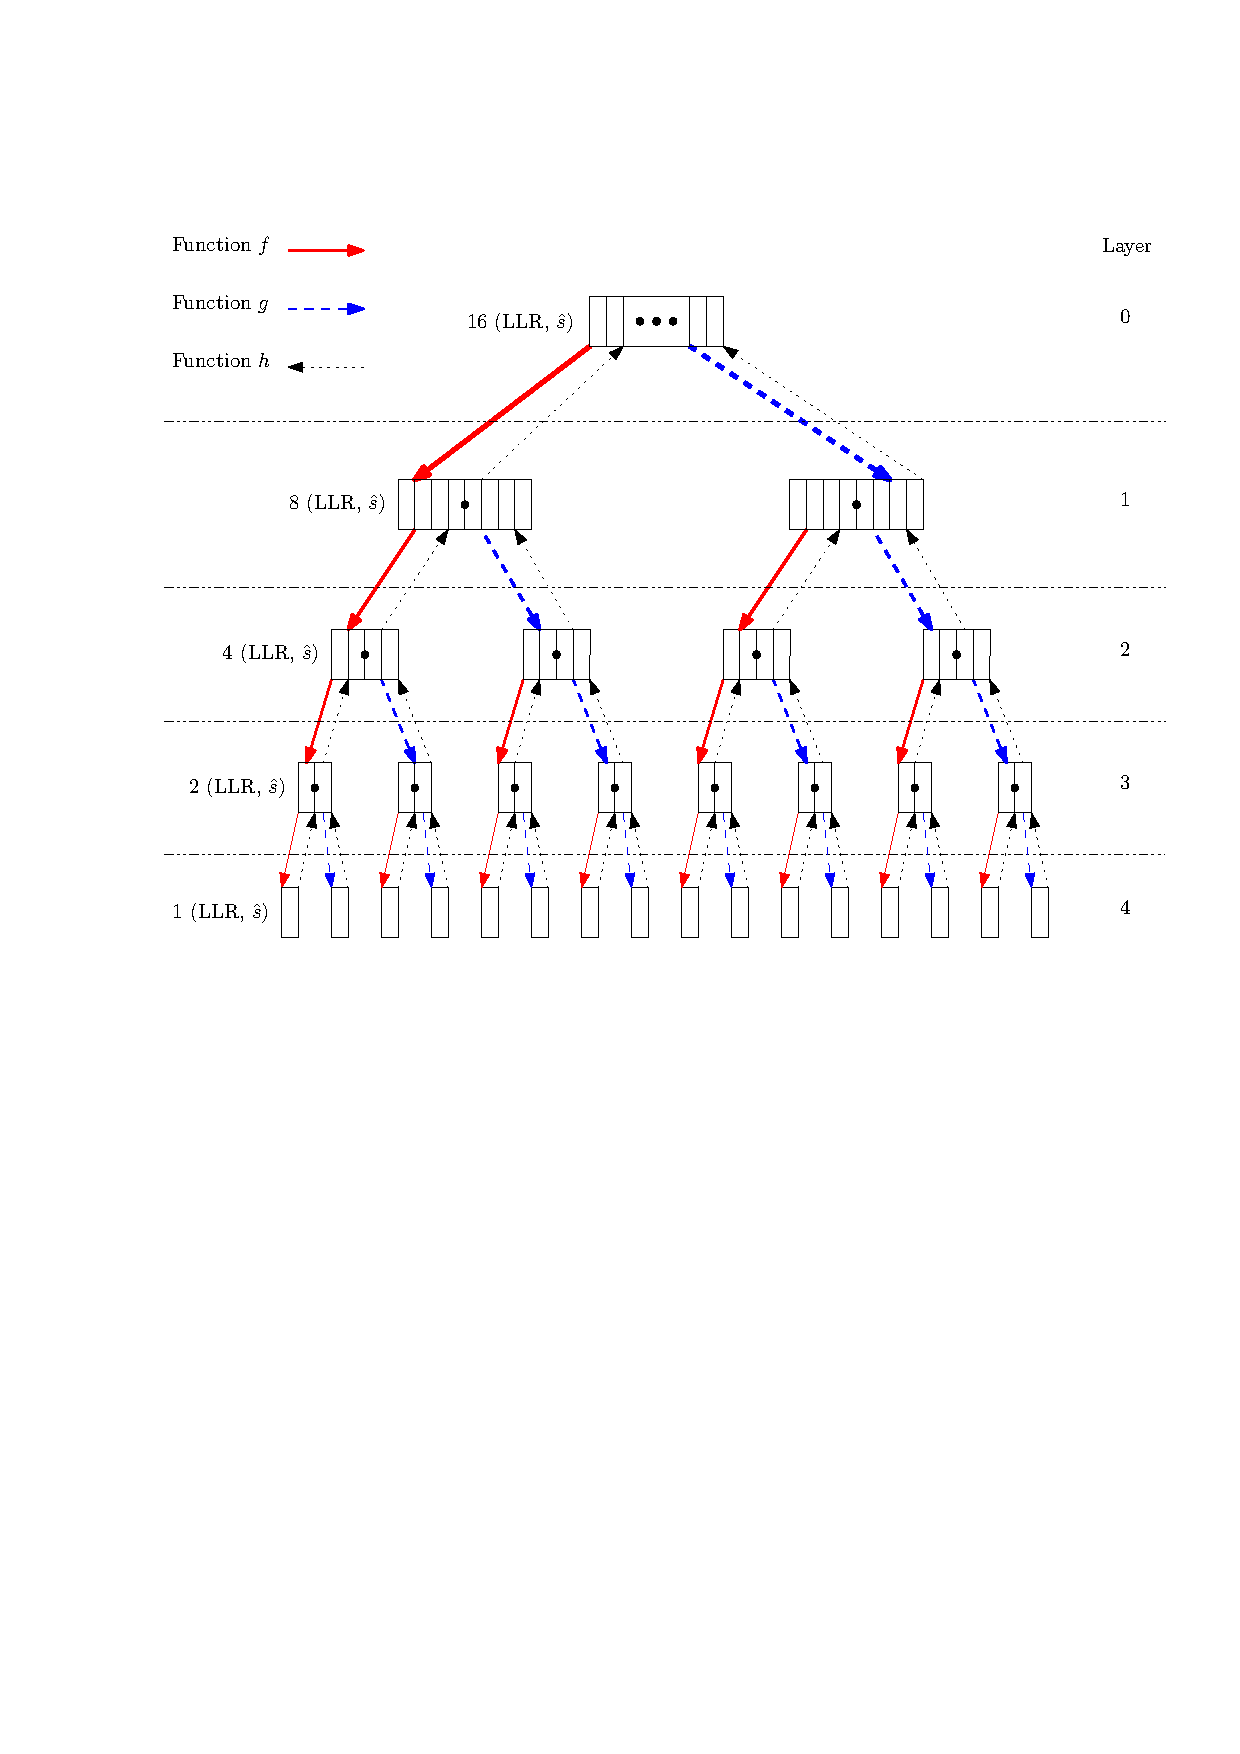
\includegraphics{\curChapter/fig/polar/sc_decoder/sc_decoder}
  \caption{Full SC decoding tree ($N = 16$).}
  \label{fig:ctx_polar_sc_decoder}
\end{figure}

A first decoding algorithm, called the Successive Cancellation (SC) decoding
algorithm, has been introduced by \Arikan~\cite{Arikan2009}. It can be seen as
the traversal of a binary tree starting from the root node. For a code length
$N=2^m$, the corresponding tree thus includes $m + 1$ node layers, indexed from
$d=0$ (root node layer) down to $d=m$ (leaf nodes layers). As the tree is
initially full, each layer $d$ contains $2^d$ nodes, each node of that layer $d$
containing $2^{m-d}$ LLRs ($\bm{\lambda}$) and $2^{m-d}$ binary values denoted
as \textit{partial sums} ($\bm{\hat{s}}$). At the decoder initialization, LLR
values received from the channel ($\bm{l}$) are stored in the root node. Then,
the decoding process performs a pre-order traversal of the tree. When a node is
visited in the downward direction, LLRs of the node are updated. In the upward
direction, partial sums are updated. Figure~\ref{fig:ctx_polar_sc_decoder}
summarizes the computations performed in both directions. The update functions
are:
\begin{eqnarray}
\left\{\begin{array}{l c l c l}
\lambda_c &=& f(\lambda_a,\lambda_b) &=& \lambda_a \boxplus \lambda_b \approx \sign(\lambda_a.\lambda_b).\min(|\lambda_a|,|\lambda_b|)\\
\lambda_c &=& g(\lambda_a,\lambda_b,\hat{s})&=&(1-2\hat{s})\lambda_a+\lambda_b\\
(\hat{s}_{c}, \hat{s}_{d}) &=& h(\hat{s}_{a}, \hat{s}_{b}) &=& (\hat{s}_{a} \oplus \hat{s}_{b}, \hat{s}_{b}).
\end{array}\right.
\label{eq:ctx_polar_f_g_h}
\end{eqnarray}
The $f$ and $g$ functions both generate a single LLR. The $h$ function provides
a couple of partial sums. The $f$ function is the Min-Sum approximation of the
$\boxplus$ operation described in Equation~\ref{eq:ctx_ldpc_ms}. In Polar
decoding using an MS approximation does not significantly impact the decoding
performance. Thus, the MS approximation is widely applied.

Before recursively calling itself on the left node, the algorithm applies the
$f$ function, respectively. Before calling itself on the right node the $g$
function is applied. At the end (after the recursive call on the right node) the
$h$ function is applied. The $f$ and $g$ functions operate on the LLRs (read
only mode) from the current node $n_i$ in order to produce the new LLR values
into left and right $n_{i+1}$ nodes, respectively. The $h$ function reads the
bits from the left and right $n_{i+1}$ nodes in order to update the bit values
of the $n_i$ node. The $\bm{\lambda}$ LLRs in the leafs are converted in the
$\bm{\hat{s}}$ bits with the hard decision function $\hat{s}_n =
\hardDec(\lambda_n)$.

Leaf nodes are of two kinds: \emph{information bit} nodes and \emph{frozen bit}
nodes. When a frozen bit leaf node is reached, its binary value is
unconditionally set to zero. Instead, when an information leaf node is reached,
its binary value is set according to the \emph{sign} of its LLR (0 if LLR is
positive, 1 otherwise). Once every node in the tree has been visited in both
directions, the algorithm eventually updates partial sums in the root node and
the decoding process is terminated. If the polar code is not systematic, the
decoded bits $\bm{\hat{u}}$ are the leaf bits in the tree. Otherwise, if the
polar code is systematic, the decoded bits $\bm{\hat{u}}$ can be directly
extracted from the root node of the polar tree in the form of an $N$-bit partial
sum vectors. In this thesis, only the systematic polar encoding scheme is
considered. This construction leads to an improved BER while the decoding
computational complexity remains unchanged.

The SC algorithm is a key to construct the polar codes. A density evolution
is performed over the SC binary tree to determine the efficient position of the
frozen bits. The idea is to construct the polar codes according to the decoder
structure. In this manuscript, the Gaussian Approximation (GA) of the density
evolution is used~\cite{Trifonov2012}.

\subsubsection{Successive Cancellation List Decoding Algorithm}

\begin{algorithm}
  \caption{SCL decoding algorithm.}\label{alg:ctx_polar_scl_decoder}

  \SetKwProg{Fn}{Function}{}{}

  \KwData{$\lambda$ is a 2D buffer ($[L][2N]$) to store the LLRs.}
  \KwData{$\hat{s}$ is a 2D buffer ($[L][N]$) to store the bits.}

  \Fn(\Comment*[f]{$o_{\lambda}$ and $o_{\hat{s}}$ are offsets in $\bm{\lambda}$ and $\bm{\hat{s}}$, resp.}){$\SCLDecode(N, o_{\lambda}, o_{\hat{s}})$}
  {
    $N_{\frac{1}{2}} \gets N / 2$

    \uIf(\Comment*[f]{not a leaf node}){$N > 1$}
    {
      \For(\Comment*[f]{loop over the $L$ paths}){$p=0$ \textbf{to} $L-1$}
      {
        \For(\Comment*[f]{apply the $f$ function}){$i=0$ \textbf{to} $N_{\frac{1}{2}}-1$}
        {
          $\lambda[p][o_\lambda + N + i] \gets f(\lambda[p][o_\lambda + i], \lambda[p][o_\lambda + N_{\frac{1}{2}} + i])$
        }
      }

      $\SCLDecode(N_{\frac{1}{2}}, o_{\lambda} + N, o_{\hat{s}})$ \Comment*[r]{recursive call to the decoder}

      \For{$p=0$ \textbf{to} $L-1$}
      {
        \For(\Comment*[f]{apply the $g$ function}){$i=0$ \textbf{to} $N_{\frac{1}{2}}-1$}
        {
          $\lambda[p][o_\lambda + N + i] \gets g(\lambda[p][o_\lambda + i], \lambda[p][o_\lambda + N_{\frac{1}{2}} + i], \hat{s}[p][o_{\hat{s}} + i])$
        }
      }

      $\SCLDecode(N_{\frac{1}{2}}, o_{\lambda} + N, o_{\hat{s}} + N_{\frac{1}{2}})$ \Comment*[r]{recursive call to the decoder}

      \For{$p=0$ \textbf{to} $L-1$}
      {
        \For(\Comment*[f]{update the partial sums ($h$ function)}){$i=0$ \textbf{to} $N_{\frac{1}{2}}-1$}
        {
          $\hat{s}[p][o_{\hat{s}} + i] \gets h(\hat{s}[p][o_{\hat{s}} + i], \hat{s}[p][o_{\hat{s}} + N_{\frac{1}{2}} + i])$
        }
      }
    }
    \Else(\Comment*[f]{a leaf node})
    {
      $\updatePaths()$ \Comment*[r]{update, create and delete paths}
    }
  }

  $\SCLDecode(N, 0, 0)$ \Comment*[r]{launch the decoder}

  $\selectBestPath()$
\end{algorithm}

The Successive Cancellation List (SCL) algorithm is an evolution of the
SC~\cite{Tal2011}. The SCL algorithm is summarized in
Algorithm~\ref{alg:ctx_polar_scl_decoder}. Unlike the SC algorithm, the SCL
algorithm builds a list of candidate codewords along the decoding process. At
each call of the ``$\updatePaths()$'' sub-routine (l.16), $2L$ candidates are
generated. A path metric is then evaluated to keep only the $L$~best candidates
among the $2L$ paths. The path metrics are calculated as
in~\cite{Balatsoukas-Stimming2015}. At the end of the decoding process, the
candidate codeword with the best path metric is selected in the
``$\selectBestPath()$'' sub-routine (l.18). The decoding complexity of the
SCL algorithm grows as $O(LN\log_2N)$. This linear complexity in L leads to
significant improvements in BER/FER performances compared to the SC decoder,
especially for small code lengths.

The authors in~\cite{Tal2011} observed that when a decoding error occurs, the
right codeword is often in the final list, but not with the best path metric.
They proposed to concatenate a CRC to the codeword in order to discriminate the
candidate codewords at the final stage of the SCL decoding. Indeed, this
technique drastically improves the FER performance of the decoding process. This
algorithm is denoted as the \emph{CRC-Aided SCL} (CA-SCL). In terms of
computational complexity, the overhead consists in the computation of $L$ CRCs
at the end of each decoding.

\subsubsection{Simplified Successive Cancellation Class of Algorithms}
\label{sec:ctx_polar_simplified_decoders}

\begin{figure}[htp]
  \centering
  \includegraphics{\curChapter/fig/polar/tree_pruning_example/tree_pruning_example}
  \caption
    [Example of polar tree pruning on a small binary tree ($N = 8$).]
    {Example of tree pruning on a small binary tree ($N = 8$). The tree is cut
    and the computations are versioned according to the location of the frozen
    bits.}
  \label{fig:ctx_polar_tree_pruning_example}
\end{figure}

Frozen bits fully define the decoder leaf values. Hence some parts of the
traversal can be cut and its computation avoided, depending on the location of
the frozen bits. More generally, the tree functions can be versioned depending
on these bits. In~\cite{Alamdar-Yazdi2011}, a tree pruning technique called the
Simplified SC (SSC) was applied to SC decoding algorithm. An improved version
was proposed in~\cite{Sarkis2014a}. This technique relies on the fact that,
depending on the frozen bits location in the leaves of the tree, the definition
of dedicated nodes enables to prune the decoding tree: Rate-0 nodes (\verb|R0|)
correspond to a sub-tree whose all leaves are frozen bits, Rate-1 nodes
(\verb|R1|) correspond to a sub-tree in which all leaves are information bits,
REPetition (\verb|REP|) and Single Parity-Check (\verb|SPC|) nodes correspond to
repetition and SPC codes sub-trees, respectively. These special nodes,
originally defined for SC decoding, can be employed in the case of SCL decoding
as long as some modifications are made in the path metric
calculation~\cite{Sarkis2016}. This tree-pruned version of the algorithm is
called Simplified SCL (SSCL) and CA-SSCL when a CRC is used to discriminate
the final candidate codewords. The tree pruning technique can drastically reduce
the amount of computations in the decoding process. The
Figure~\ref{fig:ctx_polar_tree_pruning_example} shows that more than half of the
tree nodes can be removed for $N = 8$ and $R = 1 / 2$ (this is representative of
real-life codes).

\subsubsection{Adaptive Successive Cancellation List Decoding Algorithm}
\label{sec:ctx_polar_ascl}

The presence of the CRC can be further used to reduce the decoding time by
gradually increasing $L$. This variation of SCL is called Adaptive SCL
(A-SCL)~\cite{Li2012}. The first step of the A-SCL algorithm is to decode the
received frame with the SC algorithm. Then, the decoded polar codeword is
checked with a CRC. If the CRC is not valid, the SCL algorithm is applied with
$L=2$. If no candidate in the list satisfies the CRC, $L$ is repeatedly doubled
until it reaches the value $L_{max}$. We call this version of the A-SCL decoding
the Fully Adaptive SCL (FA-SCL) as opposed to the Partially Adaptive SCL
(PA-SCL), in which the $L$ value is not gradually doubled but directly increased
from $1$ (SC) to $L_{max}$. The simplified versions of these algorithms are
denoted PA-SSCL and FA-SSCL. In order to simplify the algorithmic range, in the
remainder of the manuscript, only the simplified versions are considered. The
use of either the FA-SSCL or the PA-SSCL algorithmic improvement introduces no
BER or FER performance degradation as long as the CRC length is adapted to the
polar code length. If the CRC length is too short, the decoding performance may
be degraded because of false detections. These adaptive versions of SSCL can
achieve higher throughputs. Indeed, a large proportion of frames can be decoded
with a single SC decoding. This is especially true when the SNR is high.

\subsection{Turbo Codes}
\label{sec:ctx_turbo}

\subsubsection{Coding Scheme}

In this sub-section, the convolutional sub-encoder is presented first and then
the turbo encoding process is detailed. The first convolutional codes have been
introduced by Peter Elias in 1955~\cite{Elias1955}. The objective was to propose
an alternative to block codes in term of codeword length flexibility:
theoretically, the length of a convolutional code is infinite. The coding scheme
output depends on the current input and on the few previous inputs.

\begin{figure}[htp]
  \centering
  \subfloat[][Encoder scheme.]
  {
    \includegraphics[scale=1.0]{\curChapter/fig/turbo/sub_encoder/sub_encoder}
    \label{fig:ctx_turbo_sub_encoder_graph}
  }
  \quad
  \subfloat[][Finite state machine.]
  {
    \includegraphics[scale=0.75]{\curChapter/fig/turbo/mealy/mealy}
    \label{fig:ctx_turbo_sub_encoder_mealy}
  }
  \\
  \subfloat[][Trellis representation.]
  {
    \includegraphics[scale=0.9]{\curChapter/fig/turbo/trellis/trellis}
    \label{fig:ctx_turbo_sub_encoder_trellis}
  }
  \caption{Different representations of a recursive and systematic convolutional
           code ($R = 1/2$).}
  \label{fig:ctx_turbo_sub_encoder}
\end{figure}

For a $R=1/2$ encoder, the current $p_k$ output parity bit can be expressed as a
linear combination of the $\nu$ previous bits of the message:
$p_k = \sum_{j=0}^\nu g^{(2)}_{j} u_{k-j} + \sum_{j=1}^\nu g^{(1)}_{j} p_{k-j}$,
where $\nu$ represents the number of elements memorized inside the encoder.
The sequence of elements~$g_j$ is called the code-generating sequence and is
often expressed in octal. Figure~\ref{fig:ctx_turbo_sub_encoder_graph} gives
three representations of a convolutional code of rate $R = 1/2$ with a memory
$\nu = 2$ ($D_0$ and $D_1$ are shift registers). Its two code-generating
sequences $\bm{g^{(1)}} = (7)_8$ and $\bm{g^{(2)}} = (5)_8$ define the $c_2 = p$
output while $c_1 = u$. In the example, the convolutional code has the
particularity to be systematic because $c_1 = u$ and recursive because of the
feedback loop before the first shift register $D_0$. In the literature, this
type of coding scheme is called Recursive Systematic Convolutional (RSC). Only
RSC codes are considered in the document. In
Figure~\ref{fig:ctx_turbo_sub_encoder}, the number of $D$ memories $\nu = 2$ so,
the code can have $2^\nu = 4$ different states. Thus, a convolutional code can
be expressed as a finite-state machine as shown in
Figure~\ref{fig:ctx_turbo_sub_encoder_mealy}. The initial state $S_0$
corresponds to $D_0 = 0$ and $D_1 = 0$, the state~$S_1$ corresponds to $D_0 = 1$
and $D_1 = 0$, the state~$S_2$ corresponds to $D_0 = 0$ and $D_1 = 1$ and,
finally, the state~$S_3$ corresponds to $D_0 = 1$ and $D_1 = 1$. The notation on
the edges is in the form of $u/c_1c_2$. For instance, from the state~$S_1$, if
the input bit $u$ is 1, then the encoder will output two bits $c_1 = 1$ and
$c_2 = 0$ and will go in the state~$S_2$. This is denoted by \emph{1/10} below
the directed edge between $S_1$ and $S_2$.

Figure~\ref{fig:ctx_turbo_sub_encoder_trellis} introduces another convenient
representation of convolutional codes: the trellis. This representation has
been used for the first time by Dave Forney in 1973~\cite{Forney1973}. It is
especially useful to facilitate the understanding of the decoding process.
Indeed, it enables to see the internal state of the encoder, its transitions,
and the temporal evolution. However, the purpose of this section is not to
detail the decoding process, it will be made in the next section. Considering
the encoder initial state $S_0$, from $t = 0$ the two next possible states are
$S_0$ and $S_1$. At $t = 1$, the encoder can be in state $S_0$ or $S_1$, so the
next possible states are $S_0$, $S_1$, $S_2$ or $S_3$. One can note that
starting from $\nu +1$ time units, the trellis pattern is repeated.

\begin{figure}[htp]
  \centering
  \includegraphics{\curChapter/fig/turbo/encoder/encoder}
  \caption{Turbo code ($R = 1/3$) with two convolutional sub-encoders and a
    $\Pi$ interleaver.}
  \label{fig:ctx_turbo_encoder}
\end{figure}

As mentioned before, a turbo code is built from two convolutional codes.
Figure~\ref{fig:ctx_turbo_encoder} shows a generic view of the turbo coding
process. In the example, the code rate of the turbo code is $R = 1/3$. This rate
is obtained from two convolutional sub-encoders of rate $R = 1/2$ (like the one
shown in Figure~\ref{fig:ctx_turbo_sub_encoder}). The two parity bits $p$ and
$p'$ are obtained from the $c_2$ outputs of the convolutional codes while the
systematic $c_1$ outputs are ignored. The first sub-encoder encodes the $u$
input bit while the second one encode the $u'$ bit. The $u'$~bit is determined
from $u$ after a $\Pi$ interleaving process. For each $u_k$ bit there is a
single $u_k'$ associated bit in the $K$ input information bits. The interleaving
process is a key point for the efficiency of a turbo code. The interleaving
process permutes the information bits from their \emph{natural
(sequential) order} into the \emph{interleaved order}. The permutation function
defines the interleaver type. The $K$ information bits in the natural order are
given to the sub-encoder 1 while the $K$ information bits in the interleaved
order are given to the sub-encoder 2.

\subsubsection{Turbo Decoding Algorithm}
\label{sec:turbo_overview}

\begin{figure}[htp]
  \centering
  \includegraphics[scale=1.0]{\curChapter/fig/turbo/decoder/decoder}
  \caption{Information exchanges in turbo decoding process.}
  \label{fig:ctx_turbo_decoder}
\end{figure}

The turbo decoder consists of two component decoders exchanging soft information
in terms of log-likelihood ratio (LLR) for each transmitted information bit
through an interleaver and a deinterleaver. Figure~\ref{fig:ctx_turbo_decoder}
illustrates the internal structure of a turbo decoder. Two Soft Input Soft
Output (SISO) decoders are represented with the interleaving process $\Pi$ and
the deinterleaving process $\Pi^{-1}$. In our work, only rate $R = 1/3$
codewords are considered. $K$ represents the number of information bits and $N$
is the codeword size: $N = K \times 3$.

\paragraph{Algorithm Outline}

Turbo decoding is carried out over several iterations. Each iteration
consists of two component decoding phases. During each phase, a component
decoder performs a maximum a posteriori (MAP) decoding based on the BCJR
algorithm~\cite{Bahl1974}, which generates so-called extrinsic LLRs given the
LLRs obtained by the detector and a priori LLRs obtained from the other
component decoder. The BCJR algorithm consists of one forward and one backward
traversal on a trellis, which are defined by the underlying code. Specifically,
to decode a codeword of $K$ information bits, the BCJR algorithm performs the
following steps: (i) the branches of the trellis are weighted from the
systematic LLRs ($\bm{L_s}$), the parity LLRs ($\bm{L_p}$) and the a priori
information ($\bm{L_a}$); (ii) in the forward traversal step, it computes $K$
sets of forward state metrics for each transmitted information bit; (iii) in the
backward traversal step, it computes $K$ sets of backward state metrics for each
transmitted information bit; (iv) to compute the extrinsic LLRs ($\bm{L_e}$),
the BCJR algorithm then combines the forward and backward state metrics. The
$\bm{L_s}$, $\bm{L_p}$, $\bm{L'_p}$ vectors of LLRs correspond to the decoder
input $\bm{l}$ split into 3 sub-sets.

\begin{algorithm}
  \caption{Pseudo-code of the BCJR decoding algorithm.}
  \label{alg:ctx_turbo_bcjr}

  \For(\Comment*[f]{(i) parallel loop}){$k=0;~k<K;~k=k+1$}
  {
    $\boldsymbol{\gamma}^k\gets \computeGamma(L_{s}^k, L_{p}^k, L_{a}^k)$
  }

  $\boldsymbol{\alpha}^0\gets \initAlpha()$

  \For(\Comment*[f]{(ii) sequential loop}){$k=1;~k<K;~k=k+1$}
  {
    $\boldsymbol{\alpha}^k\gets \computeAlpha(\boldsymbol{\alpha}^{k-1}, \boldsymbol{\gamma}^{k-1})$
  }

  $\boldsymbol{\beta}^{K-1}\gets \initBeta()$

  \For(\Comment*[f]{(iii) sequential loop}){$k=K-2;~k \geq 0;~k=k-1$}
  {
    $\boldsymbol{\beta}^k\gets \computeBeta(\boldsymbol{\beta}^{k+1}, \boldsymbol{\gamma}^{k})$
  }

  \For(\Comment*[f]{(iv) parallel loop}){$k=0;~k<K;~k=k+1$}
  {
    $L_e^k\gets \computeExtrinsic(\boldsymbol{\alpha}^k, \boldsymbol{\beta}^{k}, \boldsymbol{\gamma}^{k}, L_{s}^k, L_{a}^k)$
  }
\end{algorithm}

Algorithm~\ref{alg:ctx_turbo_bcjr} summarizes the previously enumerated steps in
a pseudo-code. $\bm{\gamma}$ are the values of the trellis branches,
$\bm{\alpha}$ are the values of the nodes in the forward traversal of the
trellis and $\bm{\beta}$ are the values of the nodes in the backward traversal
of the trellis.

\begin{figure}[htp]
  \centering
  \includegraphics[width=1.0\textwidth]{\curChapter/fig/turbo/encoder_lte/encoder_lte}
  \caption
    [Turbo LTE encoder and its associated 8-state trellis.]
    {Turbo LTE encoder and its associated 8-state trellis.
     $\bm{g^{(1)}} = (13)_8$, $\bm{g^{(2)}} = (15)_8$.}
  \label{fig:ctx_turbo_encoder_lte}
\end{figure}

In this thesis, we focus on the turbo codes of the LTE standard~\cite{ETSI2013}
(3G and 4G mobile networks). Figure~\ref{fig:ctx_turbo_encoder_lte} gives the
definition of one LTE turbo encoder. This encoder leads to an 8-state trellis.
In the next sections and chapters, this LTE trellis is always considered.

\paragraph{Branch-metric Computations}

Let $S_j^{k+1}$ be the $j^{th}$ state associated with information bit $k+1$ and
$j \in \{0,7\}$. There are two incoming branches into state $S_j^{k+1}$. Each
incoming branch is associated with values $u^k$ and $p^k$, the $k^{th}$
information bit and the parity bit (both $\pm1$), respectively. The branch
metrics associated with states $S_i^k$ and $S_j^{k+1}$ are computed as follows:
\begin{equation}
\label{eq:ctx_turbo_gamma}
 \gamma(S_i^k, S_j^{k+1}) = 0.5(L_{s}^k + L_a^k)u^k + 0.5(L_p^k p^k).
\end{equation}
$L_{s}^k$ and $L_a^k$ are the systematic channel LLR and the a priori LLR for
$k^{th}$ trellis step, respectively. In the BCJR SISO decoder 1, the
$\bm{L_{s}}$, $\bm{L_{p}}$ and $\bm{L_{a}}$ vectors of LLRs are considered
in the natural domain while in the BCJR SISO decoder 2, the $\bm{L'_{s}}$,
$\bm{L'_{p}}$ and $\bm{L'_{a}}$ LLRs are used instead in the interleaved domain.
However, the computations in the natural and in the interleaved domain are
similar. That is the reason why only the operations in the natural domain are
described here. Note that it is not necessary to evaluate the branch metric
$\gamma(s^k , s^{k+1})$ for all 16 possible branches, as there are only four
different branch metrics: $\gamma^k_0 = 0.5(L_{s}^k + L_a^k + L_p^k)$,
$\gamma^k_1 = 0.5(L_{s}^k + L_a^k - L_p^k)$, $-\gamma^k_0$, and $-\gamma^k_1$.

\paragraph{Forward and Backward State-metric Computations}

The forward state metrics have to be computed recursively from trellis step to
trellis step. The forward state metrics of step $k+1$ correspond to the vector
$\bm{\alpha^{k+1}} = [\alpha_0^{k+1}, ... ,\alpha_7^{k+1}]$, where the
$j^{th}$ forward state metric $\alpha_j^{k+1}$ only depends on two forward
state metrics of stage $k$. These state metrics are computed as:
\begin{equation}
  \label{eq:ctx_turbo_alpha}
  \alpha_j^{k+1} =
  \maxstar_{i \epsilon F} ( \alpha_i^k + \gamma(S_i^k, S_j^{k+1}) ),
\end{equation}
where the set $F$ contains the two indexes of the states in step $k$ connected
to state $S_j^{k+1}$ (as defined by the trellis). The $\maxstar$ operator can be
expressed as follow:
\begin{equation}
   \maxstar(a,b) = \max(a,b) + \log(1 + \exp(-|a-b|)),
\end{equation}
where $\log(1 + \exp(-|a-b|))$ is a correction term.
Computations of the backward state metrics are similar to that of the forward
trellis traversal in Equation~\ref{eq:ctx_turbo_alpha}. The vector of backward
state metrics, denoted by $\bm{\beta^k} = [\beta_0^k, ..., \beta_7^k]$, is
computed as:
\begin{equation}
  \label{eq:ctx_turbo_beta}
  \beta_j^k =
  \maxstar_{i \epsilon B} ( \beta_i^{k+1} + \gamma(S_j^k, S_i^{k+1}) ),
\end{equation}
where $B$ is the set containing the indexes of states in step $k+1$ connected to
state $S_j^k$ as defined by the trellis.

\paragraph{Extrinsic LLR Computations}

After the forward and backward recursions have been carried out, the extrinsic
LLRs for the $k^\text{th}$ bit are computed as follow:
\begin{equation}
  \label{eq:ctx_turbo_ext}
  \begin{aligned}
  L_e^k = \maxstar_{\{S_k, S_{k+1}\}\epsilon U^1}\big( \alpha_i^k + \beta_j^{k+1} +
  \gamma(S_i^k, S_j^{k+1}) \big) \\
  - \maxstar_{\{S_k, S_{k+1}\}\epsilon U^{-1}}\big( \alpha_i^k + \beta_j^{k+1} +
  \gamma(S_i^k, S_j^{k+1}) \big) \\
  - L_{s}^k - L_a^k,
  \end{aligned}
\end{equation}
where the sets $U^1$ and $U^{-1}$ designate the set of states connected by paths
where $u^k=1$ and the set of states connected by paths where $u^k=-1$ (BPSK
mapping), respectively.

\paragraph{Approximation of the MAP Operations in the BCJR Decoder}

The $\maxstar$ operator of the MAP algorithm is compute intensive, mainly due to
the logarithm and exponential functions in the correction term. It can be
approximated as follow: $\maxstar(a,b) \approx \max(a,b)$. The correction term
is simply removed. This approximation is called the \emph{max-log-MAP} algorithm
(ML-MAP). Its low computational complexity makes efficient software and hardware
implementations possible. However, the ML-MAP algorithm can negatively affect
the decoding performance. Yet, it is possible to partially recover the
error-rate performance loss by scaling the extrinsic LLRs in the turbo decoder
by a factor $\alpha$. This version is called the \emph{Enhanced} max-log-MAP
(EML-MAP) algorithm~\cite{Vogt2000,Studer2011}.

\section{Applicative Contexts}

In the previous section, three channel code families have been presented. In
this thesis we focus on software implementations of the previously introduced
channel decoders. These decoders can be used in different applicative contexts
such as simulations or in real-time systems for instance. This section
describes the different applicative contexts that will be considered all along
the manuscript.

\subsection{Functional Simulation}
\label{sec:ctx_simulation}

There are many possible coding schemes with different characteristics. The
previous section introduced several families of FEC codes that are present in
most of common standards. Before they were standardized, these codes have been
evaluated and compared. The codes can be applied in a infinity of different
ways. For each coding scheme, many different decoding algorithms can be
implemented. It is then mandatory to be able to evaluate and compare the BER/FER
decoding performance of selected decoders with each others before implementing
them in real systems. To this purpose, the channel coding designers use
functional simulation. On an AWGN channel, depending on the channel code, it is
possible to predict with varying degrees of computational effort the BER/FER
decoding performance of a digital communication system. For simple channel codes
like BCH, RS and convolutional codes it is possible to analytically evaluate the
performance while for more complex codes like LDPC, turbo and polar codes it
becomes more difficult to use direct methods. The solution is then to resort to
a compute intensive Monte Carlo simulation of the digital communication system.
The idea is to evaluate the performance of the system by generating many random
frames and applying random noise samples on these frames, the noisy frames are
decoded and the output sequence of bit $\bm{\hat{u}}$ is compared with the
initial information bits $\bm{u}$. The error count is then used to update the
BER/FER value until they reach a stable value.

\begin{figure}[htp]
  \centering
  \subfloat[][Specification of the simulation chain.]
  {
    \includegraphics[scale=1]{\curChapter/fig/simu/com_chain/com_chain}
    \label{fig:ctx_simu_com_chain_specs}
  }
  \\
  \subfloat[][Input simulation parameters and output BER results.]
  {
    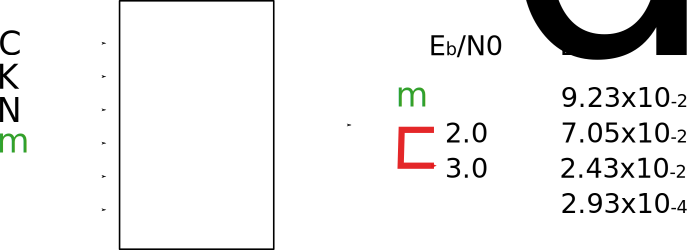
\includegraphics[scale=1]{\curChapter/fig/simu/in_out/in_out}
    \label{fig:ctx_simu_com_chain_in_out}
  }
  \caption{Description of a digital communication system simulation.}
  \label{fig:ctx_simu_com_chain}
\end{figure}

Figure~\ref{fig:ctx_simu_com_chain_specs} describes a simulation sequence
similar to the digital communication chain presented in
Figure~\ref{fig:ctx_com_chain}. The only difference is that the \emph{sink}
block has been replaced by what we call a \emph{monitor}. The \emph{monitor},
unlike the \emph{sink}, knows the $K$ output information bits from the
\emph{source} ($\bm{u}$). The $C$, $K$ and $N$ parameters define the type of
code/decoder, the number of information bits and the codeword size,
respectively. These parameters have a direct impact on the selection of the
\emph{channel encoder} and the \emph{channel decoder} blocks in the simulation.
Figure~\ref{fig:ctx_simu_com_chain_in_out} shows the BER output of the resulting
simulation. The $m$, $M$ and $s$ parameters enable to control the AWGN channel
noise. $m$ is the minimum SNR value to simulate in the channel, while $M$ is the
maximum SNR value. $s$ is the SNR step between two SNR values.

\begin{figure}[htp]
  \centering
  \subfloat[][LDPC code ($R = 5/6$).                ]{\includegraphics[width=0.475\textwidth]{\curChapter/fig/simu/bfer/bfer_ldpc}  \label{fig:ctx_bfer_ldpc}}   \quad{}
  \subfloat[][Turbo code ($R \approx 1/3$).         ]{\includegraphics[width=0.475\textwidth]{\curChapter/fig/simu/bfer/bfer_turbo} \label{fig:ctx_bfer_turbo}}  \\
  \subfloat[][Polar code ($R \approx 0.84$).        ]{\includegraphics[width=0.475\textwidth]{\curChapter/fig/simu/bfer/bfer_polar} \label{fig:ctx_bfer_polar}}  \quad{}
  \subfloat[][Turbo product code ($R \approx 0.78$).]{\includegraphics[width=0.475\textwidth]{\curChapter/fig/simu/bfer/bfer_tpc}   \label{fig:ctx_bfer_tpc}}    \\
  \subfloat[][Algebraic codes ($R \approx 0.93$).   ]{\includegraphics[width=0.475\textwidth]{\curChapter/fig/simu/bfer/bfer_bch_rs}\label{fig:ctx_bfer_bch_rs}} \quad{}
  \subfloat[][Convolutional codes ($R \approx 1/2)$.]{\includegraphics[width=0.475\textwidth]{\curChapter/fig/simu/bfer/bfer_rsc}   \label{fig:ctx_bfer_rsc}}
  \caption
    [BER and FER simulation results on various code families.]
    {BER and FER simulation results on various code families and decoder
    configurations. Lower is better. The codes are given in the $(N,K)$ form.}
  \label{fig:ctx_bfer}
\end{figure}

As an illustration, Figure~\ref{fig:ctx_bfer} presents BER and FER decoding
performances estimated with Monte Carlo simulations on a large variety of code
families and decoding parameters. On each graphic, the BER is plotted with solid
lines while the FER is plotted with dashed lines. Both the BER and the FER
depend on the SNR ($E_b/N_0$). The higher the SNR is, the lower the noise is and
therefore the number of errors. In Figure~\ref{fig:ctx_bfer_ldpc}, for instance,
on the same LDPC code ($N = 648$ and $K = 540$) and considering a 5.0 dB SNR,
the configuration 2 of the decoder achieves better decoding performance than the
configuration 1 because the {\color{Paired-3} green} curve is below the
{\color{Paired-7} orange} curve. In other terms, lower is better. When multiple
configurations are shown together, they are ordered by increasing BER/FER
performance. This is achieved at the cost of a higher computational effort
during the decoding process compared to the first configuration. The purpose of
Figure~\ref{fig:ctx_bfer} is not to compare codes with each others but to
introduce the typical BER/FER curves that will be used in the next chapters. It
shows that there is a large set of possible combinations of codes and decoding
configurations.

\newpage
\subsection{Software-defined Radio}

A Software-Defined Radio (SDR) is a radio communication system where components
traditionally implemented in hardware are instead implemented by means of
software. The concept was first introduced by Joseph Mitola in
1992~\cite{Mitola1992,Mitola1993}. Since then, SDR systems have been used in
various contexts such as military needs or amateur radio for instance. Recently,
the SDR is considered a good candidate for the 5G wireless mobile network and
more generally in cloud radio access networks. This is detailed in the next
paragraphs.

A cellular network or mobile network is a communication network where the last
link is wireless. The principle of mobile networks is to divide the territory
into zones called ``cells''. Each cell is associated to a base station and a
number of frequency channels to communicate with mobile terminals. Each base
station is connected to the networks handling voice calls, text messages and
data transfers. As standards evolve, the structure of mobile networks changes in
order to increase throughput and latency performance and also the number of
connected terminals. The objective is to cope with the exponential growth of
terminals.

\begin{figure}[htp]
  \centering
  \subfloat[][Early base station.]{\includegraphics[scale=0.715]{\curChapter/fig/sdr/base_station/base_station_1G_2G} \label{fig:ctx_sdr_base_station_1G_2G}}
  \quad{}
  \subfloat[][BB and RF processing separation.]{\includegraphics[scale=0.715]{\curChapter/fig/sdr/base_station/base_station_3G_4G} \label{fig:ctx_sdr_base_station_3G_4G}}
  \quad{}
  \subfloat[][C-RAN.]{\includegraphics[scale=0.715]{\curChapter/fig/sdr/base_station/base_station_5G_future} \label{fig:ctx_sdr_base_station_5G_future}}
  \caption
    [Base stations evolution in mobile networks.]
    {Base stations evolution in mobile networks.}
  \label{fig:ctx_sdr_base_station}
\end{figure}

In the two first generations of mobile networks (1G and 2G), all the signal
processing was treated in the base station near the antenna (see
Figure~\ref{fig:ctx_sdr_base_station_1G_2G}). Since the third generation of
mobile networks (3G) two types of processing have been separated: 1) the radio
frequency (RF) processing on the one side and 2) the base band (BB) processing
on the other side. The RF processing is attached to the antenna while the BB
processing is shared among multiple antennas (see
Figure~\ref{fig:ctx_sdr_base_station_3G_4G}). The range of this type of station
is approximately 40 kilometers. The connexions between the antennas and the BB
station are made through wired links. The RF processing mainly converts the
analog signal into a digital one (or the other way around) while the BB station
performs all the digital processing including the encoding/decoding and the
digital modulation/demodulation. The purpose of separation of the RF and BB
processing is to be able to put the BB stations near the urban centers and so to
reduce their cost of maintenance.

The virtualization of the mobile network is considered by industrial
actors~\cite{Huawei2013,Ericsson2015} and academic ones~\cite{Wubben2014,
Rost2014,Checko2015a} as a promising evolution. This is also known as the
\emph{Cloud Radio Access Network} (C-RAN): it is proposed for a part of
the processing traditionally made in the base stations. In this network
structure, the computational hardware resources of the BB processing are shared
between multiple antennas (see Figure~\ref{fig:ctx_sdr_base_station_5G_future}).
This enables new optimizations: 1) better adaptation to non-uniform traffic;
2) energy saving; 3) higher throughput and lower latency; 4) scalability and
maintainability increase~\cite{Checko2015a}. Thus, the computational BB units
have to be virtualized: there should no longer be hardware dedicated to specific
antenna. Contrariwise, the BB computational effort has to be distributed at the
cloud level.

From the first to the fourth generation of mobile networks, the BB processing
was systematically made on Application-Specific Integrated Circuits (ASICs or
dedicated hardware). However, with the emergence of the C-RAN more flexible
solutions like the software ones are seriously considered. On the receiver side,
the algorithms can be compute intensive (especially the digital demodulation and
the channel decoding). Knowing that, a main challenge is to be able to achieve
high throughput and low latency software implementations as well as flexible
ones~\cite{Nikaein2015,Rodriguez2017}.

\subsection{Sparse Code Multiple Access}
\label{sec:ctx_scma}

Non-Orthogonal Multiple Access (NOMA) mechanisms are investigated as means to
improve the fifth-generation mobile communication systems (5G)~\cite{Islam2017}
to support massive connectivity and to reduce bit error rates. Sparse Code
Multiple Access (SCMA) is a NOMA mechanism that offers better bit error rate
performance and higher spectral efficiency, while the sparsity of the codebooks
ensures a lower complexity of decoding compared to other non-orthogonal
modulations~\cite{Nikopour2013}. SCMA is a promising candidate for 5G
communication systems since it provides up to 3 times more connectivity by
spreading the information of each user's codebook over sets of shared Orthogonal
Frequency-Division Multiplexing (OFDM)~\cite{Altera2015}. According to the NGMN
white paper~\cite{Alliance2015}, 5G targets more diverse scenarios compared to
4G. Applications can be broadband support in dense areas, low latency
connectivity for Augmented Reality (AR) and reliable communication for
intelligent industrial controls, Internet of Things (IoT) or Internet of Mission
Critical Things (IoMCT). Unfortunately, the massive connectivity and spectral
efficiency of SCMA come at the cost of high complexity in the decoder, making
the design of high throughput and low complexity decoders a
challenge~\cite{Lu2015}. In this thesis, we propose to study the SCMA system
as it is usually combined with the channel code families presented before.
It is introduced in this section and revised later in light of the needs of
Cloud Radio Access Networks (C-RANs).

\subsubsection{Overview of the System Model}
\label{sec:ctx_scma_overview}

In this section, scalar, vector and matrix are presented as $x$, $\bm{x}$,
$\bm{X}$ respectively. The $n^\text{th}$ element of a vector denoted by
$\bm{x}_n$ and $\bm{X}_{n,m}$ is the element of $n^\text{th}$ row and
$m^\text{th}$ column of matrix $\bm{X}$. Notation $\diag(x)$ shows a diagonal
matrix where its n'th diagonal element is $\bm{x_n}$. In addition, the transpose
of a matrix is expressed as $\bm{X^T}$.

An SCMA encoder with $J$ users (layers) and $K$ physical resources is a function
that maps a binary stream of data to $K$-dimensional complex constellations
$f : \mathbb{B}^{log_{2}(M)} \rightarrow \mathbb{X}, x = f(\bm{b})$ where
$\bm{X} \subset \mathbb{C}^k$. The $K$-dimensional complex codeword $x$ is a
sparse vector with $N < K$ non-zero entries. Each layer $j=1, ..., J$ has its
own codebook to generate the desired codeword according to the binary input
stream. Figure~\ref{fig:ctx_scma} shows the SCMA uplink chain with $J = 6$,
$K = 4$ and $N = 2$. SCMA codewords are spread over $K$ physical resources, such
as OFDM tones. Figure~\ref{fig:ctx_scma_enc} shows that in the multiplexed
scheme of SCMA, all chosen codewords of the $J$ layers are added together after
being multiplied by the channel coefficient $\bm{h}_j$. Then, the entire uplink
chain is shown in Figure~\ref{fig:ctx_scma_codec}. The output of the SCMA
encoder is altered by a white additive noise $\bm{n}$:
\begin{equation}
  \label{eq:ctx_scma_1}
  \bm{y} = \sum\limits_{j=1}^J \diag(\bm{h}_j)\bm{x}_j+\bm{n},
\end{equation}
where $\bm{x}_j=(x_1,...,x_{Kj})^T$ and $\bm{h}_j=(h_1,...,h_{Kj})^T$ are
respectively codeword and channel coefficients of layer $j$.
Considering the digital communication chain presented in
Figure~\ref{fig:ctx_com_chain} the SCMA encoder can be seen as a digital
modulator and the SCMA decoder can be seen as a digital demodulator.

\begin{figure}%[htp]
  \centering
  \subfloat[][SCMA encoder with 6 users (layers) and 4 physical resources.]{
    \label{fig:ctx_scma_enc}
    \includegraphics{\curChapter/fig/scma/codec/codec_enc}
  }
  \\
  \subfloat[][SCMA uplink chain with channel coding.]{
    \label{fig:ctx_scma_codec}
    \includegraphics{\curChapter/fig/scma/codec/codec_chain}
  }
  \\
  \subfloat[][Factor graph representation of a decoder.]{
    \label{fig:ctx_scma_dec_graph}
    \includegraphics{\curChapter/fig/scma/codec/codec_graph}
  }
  \quad
  \subfloat[][Message Passing Algorithm based on Bayesian factor graph:\linebreak
              (I)   Resource to user message,
              (II)  Guess swap at each user and user to resource message,
              (III) Final guess at each user.]{
    \label{fig:ctx_scma_dec_alg}
    \includegraphics{\curChapter/fig/scma/codec/codec_dec}
  }
  \caption
    [SCMA system model, encoding and decoding schemes.]
    {SCMA system model, encoding and decoding schemes.}
  \label{fig:ctx_scma}
\end{figure}

\subsubsection{Message Passing Algorithm Decoding Scheme}
\label{sec:ctx_scma_detection}

Exploiting sparsity of the codebooks, Message Passing Algorithm (MPA)
decoders were introduced to achieve very good decoding performance with lower
complexity~\cite{Zhang2014a}. Figure~\ref{fig:ctx_scma_dec_graph} shows a
Bayesian factor graph representation of an MPA decoder with six users and four
physical resources. Thanks to the sparsity of the codebooks, exactly three users
collide in each physical resource. There are four possible codewords for each of
the three connected user's codebooks, which gives 64 possible combined codewords
in each physical resource.

In the first step of the MPA, the 64~distances between each possible
combined codeword and the actual received codeword are calculated:
\begin{equation}
  \label{eq:ctx_scma_5}
  d_{RES  \beta}(\bm{m}, \bm{H}) =
  \underset{l \subset \zeta, m_u\in\{1,...,K\}}{||\bm{y}_\beta -
  \sum \bm{h}_{l,m_u} \bm{x}_{l,m_u} ||},
\end{equation}
where $\zeta$ is the set of users connected to resource $\beta$ and the
considered codeword is denoted as~$m$. Assuming perfect channel estimation and
Gaussian noise, these Euclidean distances can be expressed as probabilities
using \eqref{eq:ctx_scma_7}:
\begin{equation}
  \label{eq:ctx_scma_7}
  \Psi(d_{RES \beta}) = \exp \Bigg(-\frac{d_{RES \beta}^2}{2\sigma^2} \Bigg).
\end{equation}
After calculating the residual probability of each codeword with
\eqref{eq:ctx_scma_7}, iterative MPA starts exchanging beliefs on possible
received codewords among the users and resources nodes of the factor-graph.
According to Figure~\ref{fig:ctx_scma_dec_alg} (I), a message from resources to
users has been defined to contain extrinsic information of two other connected
users. For instance, a message from resource~4 to user~2 containing the
probability information of codeword $i$ can be expressed as:
\begin{equation}
  \label{eq:ctx_scma_8}
  \begin{split}
  \mu_{RES4 \rightarrow UE2}(i) = \sum\limits_{j=1}^4 \sum\limits_{i=1}^4 \Psi
  \Big(d_{RES4}(i,j,k,\bm{H}) \Big)
  \times \mu_{UE4 \rightarrow RES4}(j) \times \mu_{UE5 \rightarrow RES4}(k).
  \end{split}
\end{equation}
As shown in Figure~\ref{fig:ctx_scma_dec_alg}(II) there are only two resources
connected to each user. A message from a user to a resource is a normalized
guess swap at the user node:
\begin{equation}
  \label{eq:ctx_scma_9}
  \mu_{UE3 \rightarrow RES1}(i) = \frac{\mu_{RES3 \rightarrow UE3}(i)}
  {\sum_i\mu_{RES3 \rightarrow UE3}(i)}.
\end{equation}
Message passing between users and resources (see \eqref{eq:ctx_scma_8} and
\eqref{eq:ctx_scma_9}) will be repeated three to eight times to reach the
desired decoding performance. The final belief at each user $B(i)$ is the
multiplication of all incoming messages as illustrated in
Figure~{\ref{fig:ctx_scma_dec_alg}}(III) and \eqref{eq:ctx_scma_10} for UE3 and
codeword $i$. Finally, \eqref{eq:ctx_scma_11} is used to calculate soft outputs
for $\bm{\hat{x}}$:
\begin{equation}
  \label{eq:ctx_scma_10}
  B_3(i) = \mu_{RES1 \rightarrow UE3}(i) \times \mu_{RES3 \rightarrow UE3}(i),
\end{equation}
\begin{equation}
  \label{eq:ctx_scma_11}
  \bm{\hat{x}} = \ln \Bigg( \frac{\prob(\bm{y}|b_x=0)}{\prob(\bm{y}|b_x=1)} \Bigg) =
  \ln \Bigg( \frac{\sum_m B_m(i)_{~\text{when}~b_x=0}}{\sum_m B_m(i)_{~\text{when}~b_x=1}}
  \Bigg).
\end{equation}

\paragraph{Log-MPA}
\label{sec:ctx_scma_log-map}

Since calculation of exponentials in \eqref{eq:ctx_scma_7} requires relatively
high computational effort, changing the algorithm to logarithmic domain
simplifies \eqref{eq:ctx_scma_8} in:
\begin{equation}
  \label{eq:ctx_scma_13}
  \mu_{RES1 \rightarrow UE5}(i) = \underset{j,k=1,...,4}
  {\max \Bigg(-\frac{d_{RES1}^2(i,j,k,\bm{H})}{2\sigma^2} \Bigg)} +
  \mu_{UE2 \rightarrow RES1}(j) + \mu_{UE3 \rightarrow RES1}(k),
\end{equation}
due to elimination of exponential's high dynamic ranges, there is no need to
normalize the guess swap and $\mu_{UE3 \rightarrow RES1}(i) =
\mu_{RES3 \rightarrow UE3}(i).$ The rest of the algorithm can be expressed as
follows:
\begin{equation}
  \label{eq:ctx_scma_15}
  B_3(i) = \mu_{RES3 \rightarrow UE3}(i) + \mu_{RES1 \rightarrow UE3}(i),
\end{equation}
\begin{equation}
  \label{eq:ctx_scma_16}
  \bm{\hat{x}} = \max_i(B_m(i))_{~\text{when}~b_x=0} - \max_i(B_m(i))_{~\text{when}~b_x=1}.
\end{equation}

\paragraph{Estimated-MPA (E-MPA)}

Computation of the exponentials in \eqref{eq:ctx_scma_7} is one of the most
important bottlenecks of the MPA algorithm. It is possible to further accelerate
the computation by using proper estimations. The exact exponential computation
is not essential to produce a satisfying estimation in the MPA algorithms.
Considering that \eqref{eq:ctx_scma_7} represents a Gaussian PDF, it can be
replaced by sub-optimal bell-shaped polynomial distributions to model the noise.
It will be shown in Section~\ref{sec:eval_scma_throughput} that using a
polynomial estimation can increase the throughput while leading to marginal bit
error rate degradation after the MPA decoding. However, these estimated
probabilities cause small degradations of the FER performance after the channel
decoding. The proposed PDF must satisfy two conditions to be valid: 1) it must
be positive and lower bounded at zero, 2) its integral over $(-\infty, \infty)$
must be equal to 1. The following function is suggested to estimate the
exponentials:
\begin{equation}
  \label{eq:ctx_scma_18}
  \Psi^{'}_{d_{RES \beta}} = \frac{2 / \pi}{2\sigma^2 + 4d^4_{RES \beta}}.
\end{equation}
The computation of $\Psi^{'}$ is faster than the original
$\Psi$~\cite{Ghaffari2017,Ghaffari2019}. The probabilities produced using
\eqref{eq:ctx_scma_7} and \eqref{eq:ctx_scma_18} are normalized according to
\eqref{eq:ctx_scma_9}. Furthermore, the numerator $2/\pi$ does not play an
important role in MPA and can be uniformly eliminated from all calculations to
reduce the computational effort. Thus,
\begin{equation}
  \label{eq:ctx_scma_19}
  \Psi^{'}_{d_{RES \beta}} \approx \frac{1}{2\sigma^2 + 4d^4_{RES \beta}},
\end{equation}
can be used as a systematic replacement to the exponential calculations.

\section{Problematics}
\label{sec:ctx_problematics}

On the eve of the 5G mobile communication generation, the challenge is now to
design communication systems able to transmit huge amounts of data in a short
time, at a small energy cost, in a wide variety of environments. Researchers
work at refining existing coding schemes further, to get low residual error
rates with fast, flexible, low complexity decoding processes.

\paragraph{Functional Simulation}

The validation of a coding scheme requires to estimate its error rate
performance. Usually, no simple mathematical model exists to predict such
performance. The only practical solution is to perform a Monte Carlo simulation
of the whole chain. It means that some data are randomly generated, encoded,
modulated, noised, decoded, and the performance is then estimated by measuring
the Bit Error Rate (BER) and the Frame Error Rate (FER) at the sink. This
process has the advantage of being universal but it also leads to three main
problems:

\begin{enumerate}
  \item \textbf{Simulation time:}
    $\sim$ 100 erroneous frames have to be simulated to accurately estimate the
    FER/BER. Thus, measuring a FER of $10^{-7}$ requires the simulation of the
    transmission of $\sim100\times 10^7=10^9$ frames. Assuming a frame of
    1000~bits, the simulator must then emulate the transmission of
    $10^{12}$~bits. Keeping in mind that the decoding algorithm computational
    complexity may be significant, several weeks or months may be required to
    accurately estimate the FER/BER of a coding scheme (especially at low error
    rates).

  \item \textbf{Algorithmic heterogeneity:} A large number of channel codes have
    been designed over time. For each kind of code, several decoding
    configurations are possible. While it is straightforward to describe a
    unique coding scheme, it is more challenging to have a unified software
    description that supports all the coding schemes and their associated
    algorithms. This difficulty comes from the heterogeneity of the data
    structure necessary to describe a channel code and the associated decoder:
    turbo codes are based on trellis schemes, LDPC codes are well-defined on
    factor graphs and polar codes are efficiently decoded using binary trees.

  \item \textbf{Reproducibility:} It is usually tedious to reproduce results
    from the literature. This can be explained by the large amount of empirical
    parameters necessary to define one communication system, and the fact that
    not all of them are always reported in publications. Moreover, the simulator
    source codes are rarely publicly available. Consequently, a large amount of
    time is spent ``reinventing the wheel'' just to be able to compare to the
    state-of-the-art results.
\end{enumerate}

\paragraph{Software-defined Radio}

Moreover, the Software-Defined Radio (SDR) paradigm is now considered in real
communication systems. To match the real-time constraints, here are the main
challenges:

\begin{enumerate}
  \item \textbf{High throughput:} New applications, like the video streaming,
    can be very data-intensive. As a consequence, the compute intensive blocks
    of the transceiver have to be well optimized to reach levels of performance
    comparable with the hardware implementations.

  \item \textbf{Low latency:} Reaching high throughput is not always the major
    constraint, for instance, in audio-conferencing applications it is
    uncomfortable to perceive a delay when people are speaking.

  \item \textbf{Flexibility:} The software implementations have to be able to
    adapt to various configurations. For instance, when the SNR is changing,
    the code rate $R$ of the decoder can be switched on the fly.

  \item \textbf{Portability:} The proposed solutions can be deployed on high-end
    servers as well as on embedded low power systems. Moreover, many operating
    systems coexist, and it is important to be able to support the most famous
    ones like Windows, macOS and Linux.
\end{enumerate}
